\section{Producto}\label{cons:prod}

\subsection{Motivación: (De)construyendo el producto}
\label{cons:prod:motivacion}
Para continuar con la línea seguida en la sección \ref{cons:coprod} de coproductos, trataremos de definir la construcción de producto en una categoría con la intención de abstraernos del caso particular de la ya conocida categoría de conjuntos.

Recordemos que el producto cartesiano de dos conjuntos $X$, $Y$ se define como el conjunto de los pares $(x,y)$ donde $x \in X$, $y \in Y$. Es posible definir dos funciones que dado un par, proyecten cada uno de los elementos. El producto en Agda está dado por un record equipado con dos funciones (ver código \ref{code:record:producto}, pág \pageref{code:record:producto}).

Es nuestro objetivo pensar en las relaciones en lugar de pensar en los elementos, para así abstraernos y concluir en la definición categórica, determinando restricciones sobre los morfismos. Con esto en mente, podríamos decir que un objeto producto es uno para el cual existan morfismos de proyección que vayan del objeto en cuestión hacia cada uno de los factores.

De la misma forma que concluimos en la sección de coproductos, no cualquier objeto que cuente con dicho par de morfismos resulta ser el objeto producto. Esto resulta aún más evidente cuando pensamos en los conjuntos, ya que no cualquier conjunto que cuente con un par de funciones hacia los factores $X$ e $Y$ resulta ser el producto cartesiano $X \times Y$. Es necesario entonces establecer relaciones entre el objeto producto y cualquier otro objeto de la categoría.
Si pensamos en cualquier otro conjunto $C$ que se postule como producto cartesiano, con un par de funciones $f$, $g$ hacia $X$ e $Y$ respectivamente, ¿qué relación se puede establecer con $X\times Y$?
Notemos que una característica del producto cartesiano es que mantiene la información de los objetos factores {\it a la vez}, siendo posible volver a cada uno de ellos a través de las proyecciones. Pero otra cualidad del producto cartesiano es que no contiene más ni menos información que esa. 
En este sentido, el objeto producto es el mínimo objeto que contiene la información de los factores.\\
Cualquier otro conjunto $C$ tendrá o más o menos información de la necesaria, pero siempre existirá una única función hacia $X \times Y$ simplemente aplicando $f$ y $g$ y reuniendo el resultado en un par, como se define en el siguiente código:
\begin{agdacode}{\it Función de reunión de conjuntos}

  \ExecuteMetaData[latex/CartesianProduct.tex]{reunion}
\end{agdacode}

Cabe aclarar que a pesar que en el caso de la categoría $\Set$ estos elementos existan siempre, esto no tiene que impulsarnos a pensar que será así en cualquier categoría. Definiremos a continuación cuándo una categoría cuenta con productos. 


\subsection{Definición y formalización}

\begin{definition}\label{cat:prod}
Sean $A,B$ objetos de una categoría \C. Decimos que el objeto $A\times B$ es el {\it producto} de $A$ y $B$ si existen los morfismos 
\flecha{A\times B}{\pi_1}{A} y
\flecha{A \times B}{\pi_2}{B} 
tal que para todo otro objeto $C$ y par de morfismos $\flecha{C}{f}{A},\ \flecha{C}{g}{B}$ de la categoría, exista un único morfismo $\langle f,g \rangle$ que haga conmutar al siguiente diagrama:
\begin{center}
  \xymatrixcolsep{3pc} \xymatrixrowsep{3pc}
  \centerline{\xymatrix{ 
      & C \ar[dl]_{f} \ar[dr]^{g} \ar@{-->}[d]_{\langle f,g\rangle}& \\
      A & A \times B \ar[l]^{\pi_1} \ar[r]_{\pi_2} & B }}
\end{center}

En otras palabras, se requiere que el siguiente conjunto de ecuaciones se cumpla, para todas $f$ y $g$: 
$$
 \left \{ \begin{array}{lclr}
  \pi_1 \circ \langle f, g\rangle & \cong & f &\\ 
  \pi_2 \circ \langle f, g\rangle & \cong & g &\\
  \langle f, g\rangle & \cong & h & \quad \mbox{para toda $h$ tal que } \quad \pi_1 \circ h \cong f \quad \mbox{y}\quad \pi_2 \circ h \cong g\\
 \end{array}
 \right. 
$$
\end{definition}
\vspace{3ex}


De la misma forma que con los coproductos, cuando para todo par de objetos de una categoría existe su producto, decimos que la misma {\it cuenta con productos}.

Para completar la abstracción definiremos un morfismo auxiliar que 
mapea otros dos sobre un producto. Notar que este morfismo no forma parte de la estructura algebraica de los productos, sino que se define derivada de ella:

\begin{definition}\label{cat:mprod}
Sean $A, B, C$ y $D$ objetos de una categoría $\C$ con productos y sea el par de morfismos $\flecha{A}{f}{B}$ y $\flecha{C}{g}{D}$. Se define el morfismo producto de $f$ y $g$ como
    $$f\times g = \langle f\cdot\pi_1, g\cdot \pi_2 \rangle$$
Notar que decimos que el morfismo $f \times g$ {\it mapea} $f$ y $g$ sobre $A \times C$ puesto que:
$\flecha{A\times C}{f \times g}{B\times D}$
\end{definition}

Para formalizar esta construcción en Agda, diremos que una categoría tiene productos cuando sea posible proveer un elemento \AgdaField{Prod} que construya un objeto a partir de otros dos, junto con los morfismos de proyección que llamaremos \AgdaField{projl} y \AgdaField{projr}.
El morfismo medial de reunión \AgdaField{pair} puede pensarse como un constructor de un morfismo a partir de otros dos.

A continuación se provee una función extra, debido a su amplio uso: la función \AgdaFunction{pmap}, ya expuesta en la definición \ref{cat:mprod}. Su implementación se provee dentro del record, haciendo uso de los campos declarados.

Finalmente, el record incluye tres ecuaciones, \AgdaField{pairIdl}, \AgdaField{pairIdr} y \AgdaField{pairUnique}, cuyas pruebas también deberán proveerse a la hora de definirse instancias. Dichas ecuaciones se corresponden con las presentadas en la definición \ref{cat:prod}. Presentamos esta formalización en el código \ref{cod:hasProducts}.

\begin{agdacode}{\it Formalización de categoría con productos} \label{cod:hasProducts}

\ExecuteMetaData[latex/Cat.tex]{hasProducts}
\end{agdacode}

Dada un categoría cualquiera $\C$, proveer un elemento de tipo \AgdaRecord{HasProducts} $\C$ garantizará que dicha categoría cuente con productos, asegurando por un lado una forma de construirlos y por otro las pruebas requeridas por la definición. 

Como hemos visto en la sección de \ref{cons:prod:motivacion}, la categoría $\Set$ cuenta con productos. 
A modo de ejemplo, vemos formalizada esta aseveración en el código \ref{cod:setHasProducts}. La prueba de la unicidad de la función de reunión no se expone para no ahondar en detalles que no aportan, pero resulta trivial una vez unificadas las pruebas que toma como supuesto.

\begin{agdacode}\hspace{3ex}\label{cod:setHasProducts}
  
  \ExecuteMetaData[latex/CatSet.tex]{setHasProducts}
\end{agdacode}


\subsection{Producto de Containers}
De la misma forma que hemos procedido con los coproductos de containers, tenemos el objetivo de proveer un habitante del record \AgdaRecord{HasProducts} \AgdaFunction{$\Cont$}.

Retomando el análisis general de la construcción de productos en una categoría, hemos observado que un objeto producto incluye las informaciones de los objetos factores al mismo tiempo, siendo posible proyectar cada una de ellas. 

Dados dos containers, ¿qué container podemos construir para poder guardar los datos que guardan ambos, a la vez?
Denominaremos \AgdaFunction{Both} $C$ $D$ al container producto de $C$ y $D$.
\AgdaFunction{Both} $C$ $D$ tendrá por conjunto de formas a los pares $(c,d)$, siendo $c$ forma de $C$ y $d$, de $D$. Es decir, el conjunto de formas de \AgdaFunction{Both} $C$ $D$ no es más ni menos que el producto cartesiano entre \Sh $C$ y \Sh $D$.
Las posiciones posibles dentro de una forma $(c,d)$ serán, o bien posiciones en $c$, o bien posiciones en $d$. Es decir, las posiciones serán el resultado de la unión disjunta (definida en \ref{code:uplus}, pág \pageref{code:dext}) de las respectivas posiciones originales. 

Queda entonces definido el constructor de productos \AgdaFunction{Both} como:

\ExecuteMetaData[latex/Product.tex]{Producto}

Para proyectar la información contenida en un producto de containers, construiremos dos morfismos de containers \AgdaFunction{$\Pi_1$} y \AgdaFunction{$\Pi_2$} que para todo par de containers  vaya desde su producto hasta cada uno de ellos. Sus tipos serán entonces los siguientes:

\ExecuteMetaData[latex/Product.tex]{proj1t}
\ExecuteMetaData[latex/Product.tex]{proj2t}

Para el caso del primer morfismo proyección, la función de formas retornará el primer valor del par. Es decir, \mSh $\Pi_1$ será el morfismo \AgdaField{proj$_1$} de conjuntos.
La función de posiciones indicará de qué posición en una forma dada $(c,d)$ proviene el dato a almacenar en una posición $p$ de $c$. En este caso, indicaremos que queremos buscar dentro de las posiciones del primer conjunto. Esto es, \mPos (\AgdaFunction{Both} $C\ D \Rightarrow C$) $\{(c,d)\}\ p$  será \AgdaInductiveConstructor{inj$_1$} $p$.

\ExecuteMetaData[latex/Product.tex]{proj1d}

Análogamente podemos concluir que el segundo morfismo proyección es:

\ExecuteMetaData[latex/Product.tex]{proj2d}

El morfismo de reunión construye un producto a partir de dos morfismos de mismo origen y tendrá la siguiente signatura:
  
\ExecuteMetaData[latex/Product.tex]{pairt}

En cuanto a su funcionamiento, por un lado, la función de formas aplicará las respectivas funciones de formas de los morfismos $f$ y $g$, armando un par con los resultados. La función de posiciones decide si aplicar \mPos $f$ o \mPos $g$, según a qué posición en \AgdaFunction{Both} $C\ D$ se aplique. Esto lo logramos con la función de coreunión de conjuntos \AgdaFunction{$[\_,\_]$} dada en el código \ref{code:choice}.
Finalmente,

\ExecuteMetaData[latex/Product.tex]{paird}

La prueba de la conmutatividad de cada triángulo del diagrama de la definición la obtenemos trivialmente. El siguiente código muestra la demostración de la conmutatividad izquierda. La derecha no se expone puesto que resulta análoga.

\ExecuteMetaData[latex/Product.tex]{pairidl}

Para proveer la prueba de la unicidad del morfismo de reunión tendremos que apelar al lema de equivalencia de morfismos de containers expresado en el código \ref{morph:equivalence} (pág, \pageref{morph:equivalence}) y a los postulados de extensionalidad provistos en \ref{code:ext} (pág. \pageref{code:ext}).

\ExecuteMetaData[latex/Product.tex]{pairuni}

Finalmente, podemos proveer un habitante de \AgdaRecord{HasProducts} \AgdaFunction{$\Cont$}:

\begin{agdacode}{\it Formalización de $\Cont$ como categoría con productos} 
  
\ExecuteMetaData[latex/CatCont.tex]{hasProducts}
\end{agdacode}


\subsubsection{Ejemplos con productos de containers}

\begin{example} {\it Par de listas}\label{ex:parlistas}

  Veamos primero un caso muy sencillo de producto de containers donde los dos containers originales son listas. Los pares de listas del mismo tipo se pueden constituir como un container \AgdaDatatype{Both cList cList}. Se define a continuación un ejemplo de par de listas de naturales que llamamos \AgdaFunction{ceroAdos,tresAsiete}.

\ExecuteMetaData[latex/Examples.tex]{ll}

La primera lista del par tiene longitud \AgdaNumber{3} y la segunda, \AgdaNumber{5}. En cuanto al contenido, la primera lista alberga los naturales asociados a cada posición en la lista. Es decir, es la lista del cero al dos. La segunda le suma \AgdaNumber{3} al índice en la lista, por lo que resulta ser la lista del tres al siete.

\end{example}

\begin{example}{\it Concatenación de listas}\label{example:append}

  El producto de containers resultará útil para los casos donde queramos definir morfismos que tomen como argumento más de un container, siempre que los elementos almacenados en cada uno de ellos sea el mismo. Por ejemplo, la función de concatenación toma dos listas del mismo tipo y construye otra con los elementos de las dos primeras dispuestas de forma contigua. Podemos construir un morfismo:

  \ExecuteMetaData[latex/Examples.tex]{appendt}

  La longitud de la nueva lista será la suma de las longitudes de las listas originales. 

  \ExecuteMetaData[latex/Examples.tex]{appendd}

  Dadas dos listas de longitudes $n_1$ y $n_2$, un índice $i$ en la nueva lista de longitud $(n_1 + n_2)$ se corresponderá con una posición de la primera si $i$ es menor a su longitud $n_1$, en otro caso habrá que buscar el contenido en la segunda lista. Este trabajo lo realiza la función \AgdaFunction{splitFin}, que convierte un elemento de \AgdaDatatype{Fin} $(n_1 + n_2)$ en, o bien uno de tipo \AgdaDatatype{Fin} $n_1$, o bien uno de tipo \AgdaDatatype{Fin} $n_2$.

  \ExecuteMetaData[latex/Examples.tex]{splitFin}

  La figura \ref{fig:append} expone cómo se realiza la concatenación de los containers de listas de longitud uno y tres. En la parte superior vemos los containers de listas originales y en la parte inferior, el container resultante. 

\begin{figure}[H]
    \begin{center}
  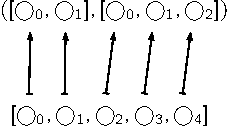
\includegraphics{img/append.pdf}
    \end{center}
    \label{fig:append}
    \caption{Concatenación de containers de listas}
\end{figure}

La reubicación de posiciones se representa en la figura con la flechas. De esta forma, para el caso particular del ejemplo, la función \AgdaFunction{splitFin} reubicará las posiciones de la siguiente manera:  
  \begin{align*}
\AgdaFunction{splitFin}\ 0 &= \AgdaInductiveConstructor{inj$_1$}\ {0}\\
\AgdaFunction{splitFin}\ 1 &= \AgdaInductiveConstructor{inj$_1$}\ {1}\\
\AgdaFunction{splitFin}\ 2 &= \AgdaInductiveConstructor{inj$_2$}\ {0}\\      
\AgdaFunction{splitFin}\ 3 &= \AgdaInductiveConstructor{inj$_2$}\ {1}\\
\AgdaFunction{splitFin}\ 4 &= \AgdaInductiveConstructor{inj$_2$}\ {2}
  \end{align*}
  
  Si extendemos el morfismo \AgdaFunction{append} sobre los naturales, obtendremos una función de pares de listas de naturales en listas de naturales. Podemos aplicar esta función al par de listas del ejemplo \ref{ex:parlistas} y obtener una lista del cero al siete.
  
\ExecuteMetaData[latex/Examples.tex]{l}

Para convertir una lista de tipo \AgdaDatatype{List} en una definida inductivamente para así poder observar y analizar los resultados más simplemente, contamos con la siguiente función:

\ExecuteMetaData[latex/Examples.tex]{tolist}

Al evaluar \AgdaFunction{ListTo[] ceroAsiete} obtenemos efectivamente una lista de naturales del cero al siete:

\AgdaNumber{0} \cons (\AgdaNumber{1} \cons (\AgdaNumber{2} \cons (\AgdaNumber{3} \cons (\AgdaNumber{4} \cons (\AgdaNumber{5} \cons (\AgdaNumber{6} \cons (\AgdaNumber{7} \cons \AgdaInductiveConstructor{[]})))))))

\end{example}
